\documentclass{beamer}
\usepackage[utf8]{inputenc}
\usepackage{amsmath}
\usepackage{graphicx}
\usepackage{xcolor}
\usepackage{tikz}

\usetheme{Madrid}
\usecolortheme{default}

% Define custom colors inspired by Star Trek DS9
\definecolor{ds9blue}{RGB}{25,25,112} % Midnight Blue
\definecolor{ds9gold}{RGB}{218,165,32} % Goldenrod
\definecolor{ds9grey}{RGB}{105,105,105} % Dim Gray
\definecolor{ds9red}{RGB}{178,34,34} % Firebrick

% Customize the colors
\setbeamercolor{title}{fg=ds9gold}
\setbeamercolor{frametitle}{bg=ds9blue, fg=white}
\setbeamercolor{block title}{bg=ds9gold, fg=black}
\setbeamercolor{block body}{bg=ds9grey!20, fg=black}
\setbeamercolor{section in toc}{fg=ds9gold}
\setbeamercolor{subsection in toc}{fg=ds9gold!70}
\setbeamercolor{footline}{bg=ds9blue, fg=white}
\setbeamercolor{author in head/foot}{fg=white}
\setbeamercolor{date in head/foot}{fg=white}
\setbeamercolor{title in head/foot}{fg=white}

% Title page configuration
\title[System \& Free Body Diagrams]{System and Free Body Diagrams}
\subtitle{A Systematic Approach to Force Diagrams\\http://newsletter.oapt.ca/files/Systems-and-FB-Diagrams.html}
\author[E. Haller]{Eric Haller}
\date[2015]{Originally published: October 25, 2015}



\AtBeginSection[]
{
  \begin{frame}
    \frametitle{Table of Contents}
    \tableofcontents[currentsection]
  \end{frame}
}

\begin{document}

\frame{\titlepage}

\begin{frame}
\frametitle{Opening Quote}
\begin{quote}
``When asked to draw a force diagram for some simple situation, most students emerging from any level of introductory physics course are likely to draw objects which look like a porcupine shot by an Indian hunting party—the number and direction of pointed entities being essentially stochastic.''
\end{quote}
\vspace{0.5cm}
\hfill -- Arnold Arons (1979)
\begin{figure}[H]
    \centering
    
\includegraphics[width=0.5\linewidth]{CH4/Porcupinebros.jpg}
\end{figure}
\end{frame}

\section{System Diagrams}

\begin{frame}
\frametitle{How to Draw System Diagrams}
\begin{enumerate}
    \item \textbf{Draw a simple sketch}
    \begin{itemize}
        \item Keep it simple
        \item Use stick figures when possible
        \item Include important elements (ground, ropes, springs)
    \end{itemize}
    \item \textbf{Draw a closed curve}
    \begin{itemize}
        \item Enclose object of interest
        \item Curve should hug object closely
        \item Label inside as "system", outside as "environment"
    \end{itemize}
\end{enumerate}
\begin{figure}
    \centering
    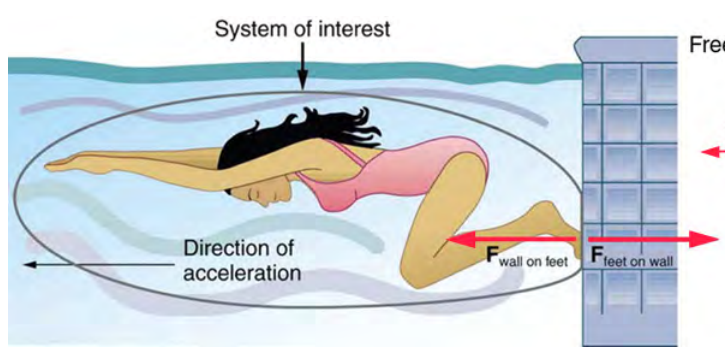
\includegraphics[width=0.5\linewidth]{Screenshot 2024-11-07 105535.png}
\end{figure}

\end{frame}

\begin{frame}
\frametitle{System Diagrams (continued)}
\begin{enumerate}\setcounter{enumi}{2}
    \item \textbf{Label contact forces}
    \begin{itemize}
        \item Identify forces at system-environment boundary
        \item Name both objects involved
        \item Multiple forces may exist at one point
    \end{itemize}
    \item \textbf{Label non-contact forces}
    \begin{itemize}
        \item Include gravity
        \item Include electromagnetic forces
        \item Write these as an aside
    \end{itemize}
\end{enumerate}

\end{frame}

\begin{frame}
\frametitle{System Diagrams (continued)}
\begin{enumerate}\setcounter{enumi}{2}
    \item \textbf{Label contact forces}
    \begin{itemize}
        \item Identify forces at system-environment boundary
        \item Name both objects involved
        \item Multiple forces may exist at one point
    \end{itemize}
    \item \textbf{Label non-contact forces}
    \begin{itemize}
        \item Include gravity
        \item Include electromagnetic forces
        \item Write these as an aside
    \end{itemize}
\end{enumerate}
\begin{figure}[H]
    \centering
    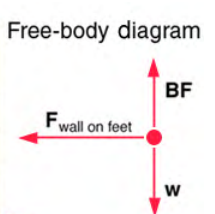
\includegraphics[width=0.3\linewidth]{Screenshot 2024-11-07 105554.png}
\end{figure}
\end{frame}

\begin{frame}
\begin{figure}[H]
    \centering
    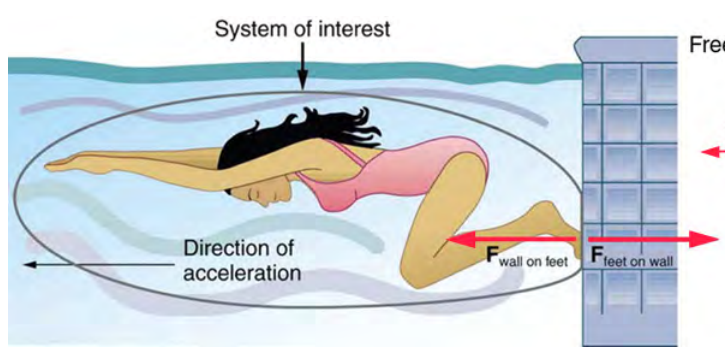
\includegraphics[width=0.5\linewidth]{Screenshot 2024-11-07 105535.png}
\end{figure}
\begin{figure}[H]
    \centering
    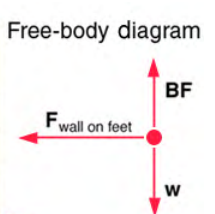
\includegraphics[width=0.3\linewidth]{Screenshot 2024-11-07 105554.png}
\end{figure}

\end{frame}

\section{Free Body Diagrams}

\begin{frame}
\frametitle{How to Draw Free Body Diagrams}
\begin{enumerate}
    \item \textbf{Draw a dot}
    \begin{itemize}
        \item Represents "the system"
        \item Makes all diagrams uniform
        \item Easier to grade and understand
    \end{itemize}
    \item \textbf{Draw force arrows}
    \begin{itemize}
        \item Start from the central dot
        \item Draw to scale when possible
        \item Include only forces from system diagram
        \item Label each force clearly
    \end{itemize}
\end{enumerate}
\begin{figure}
    \centering
    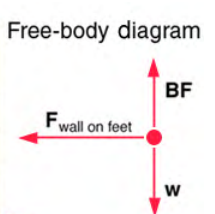
\includegraphics[width=0.2\linewidth]{Screenshot 2024-11-07 105554.png}
\end{figure}
\end{frame}

\section{Why System \& Free Body Diagrams Matter}

\begin{frame}
\frametitle{Why Do We Need These Diagrams?}
\begin{columns}
\column{0.6\textwidth}
\textbf{Key Benefits:}
\begin{enumerate}
    \item They help us organize our thoughts about forces
    \item They prevent us from forgetting forces
    \item They make solving problems easier
\end{enumerate}

\vspace{0.3cm}
\textbf{Remember:}
\begin{itemize}
    \item Always choose your system first
    \item Label ALL forces clearly
    \item Show contact and non-contact forces
\end{itemize}

\end{columns}
\end{frame}

\begin{frame}
\frametitle{Tips for Success}
\textbf{Your Diagram Checklist:}
\begin{enumerate}
    \item Start with a simple sketch
    \begin{itemize}
        \item[\Square] Keep it neat
        \item[\Square] Include only what matters
    \end{itemize}
    
    \item Label everything clearly
    \begin{itemize}
        \item[\Square] All forces named
        \item[\Square] Direction shown
    \end{itemize}
    
    \item Check your work
    \begin{itemize}
        \item[\Square] Did you include gravity?
        \item[\Square] Are contact points marked?
    \end{itemize}
\end{enumerate}

\end{frame}

\begin{frame}
\frametitle{Example Application}
\textbf{Tow Truck Scenario:}
\begin{itemize}
    \item System: Car being towed
\begin{figure}[H]
    \centering
    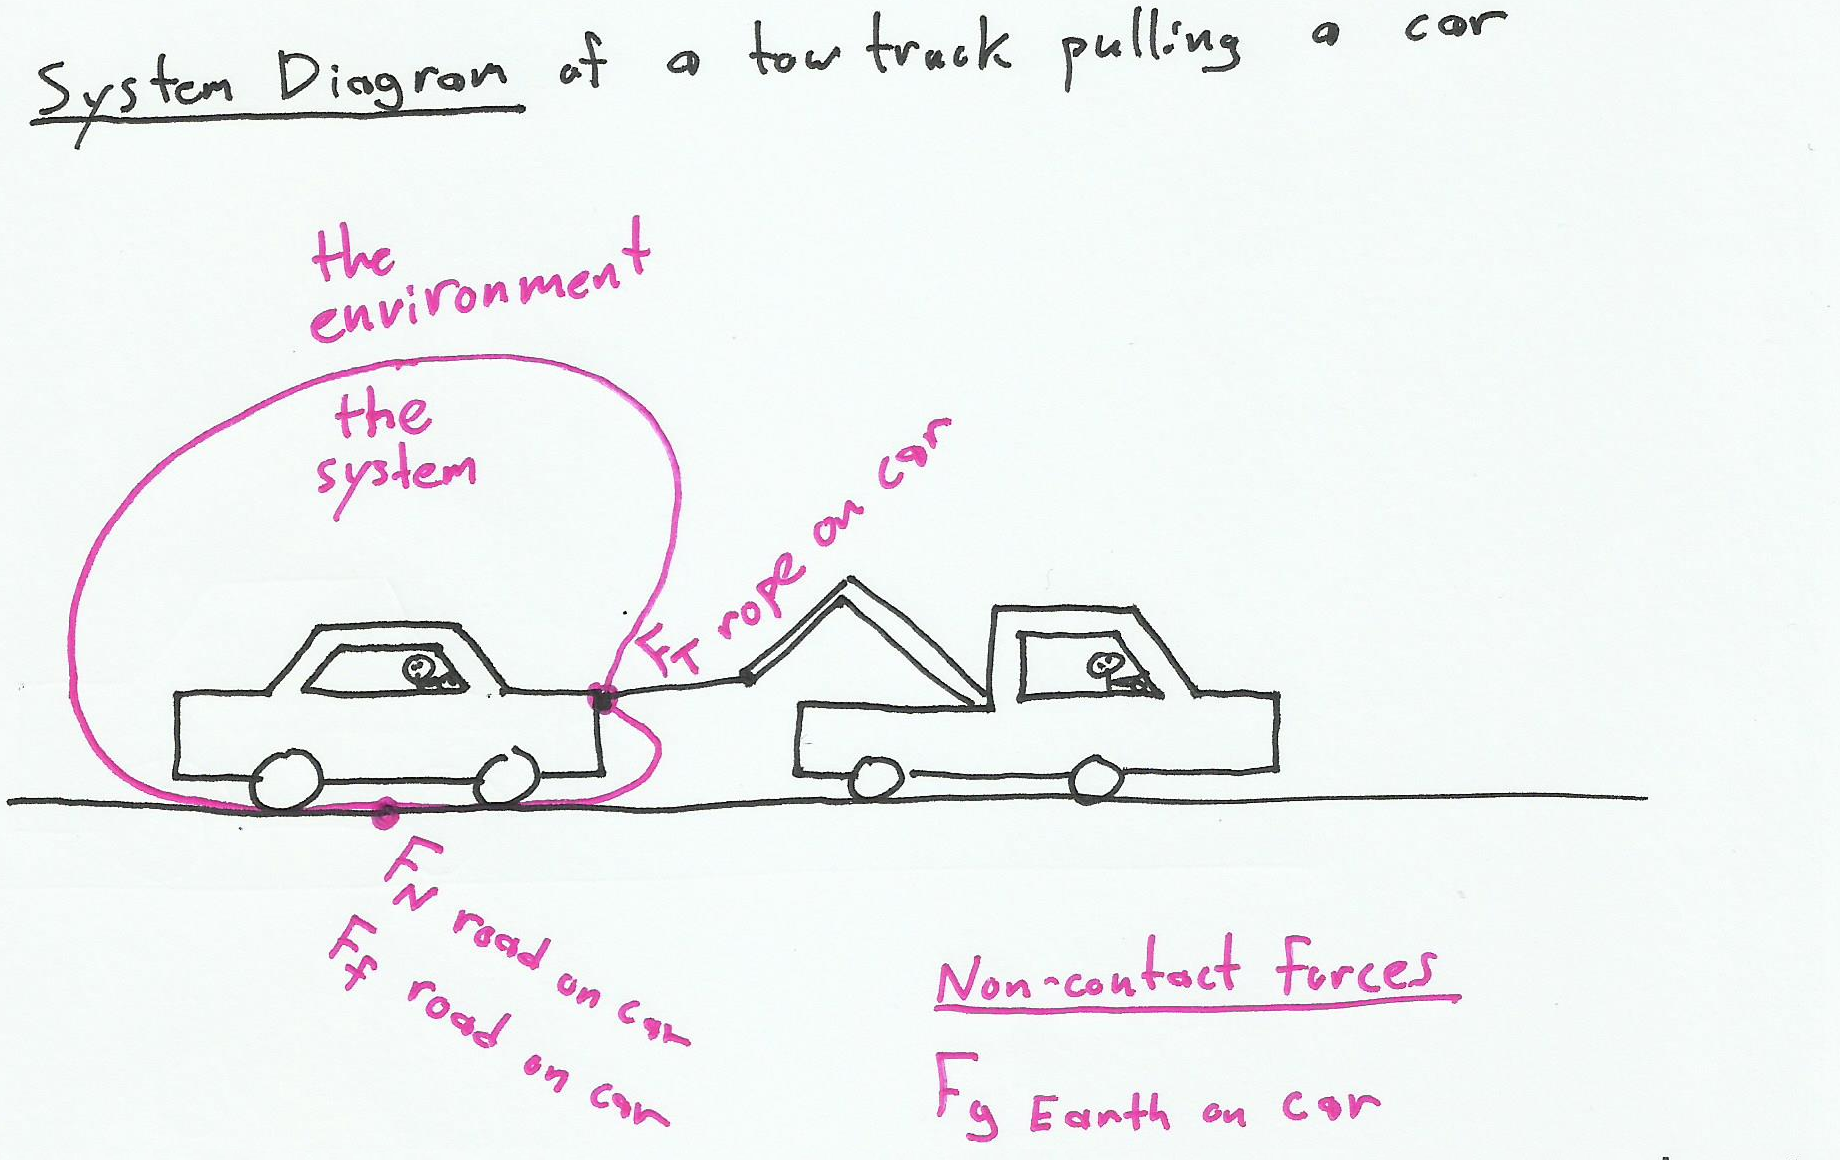
\includegraphics[width=1\linewidth]{CH4/towtruck.png}
\end{figure}
\end{itemize}

\end{frame}

\begin{frame}
\begin{figure}[H]
    \centering
    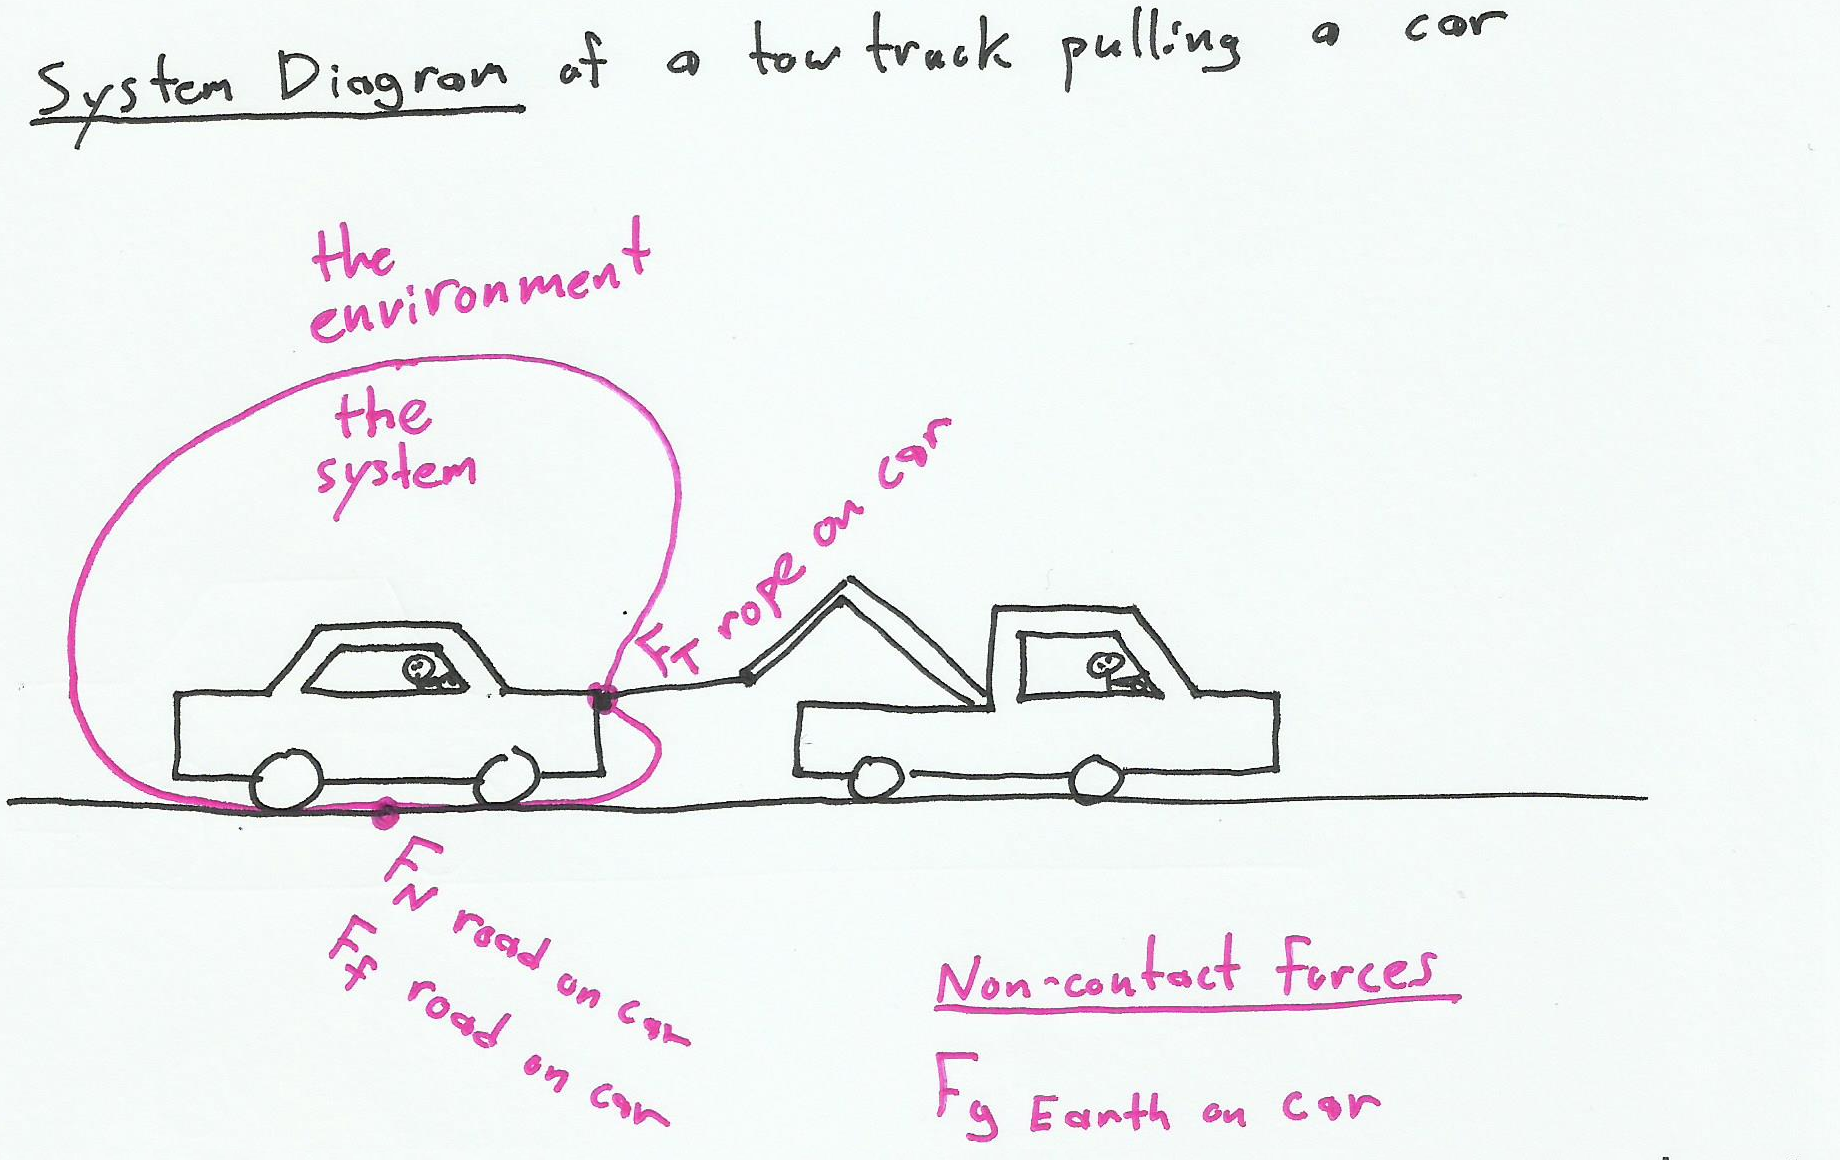
\includegraphics[width=0.7\linewidth]{CH4/towtruck.png}
\end{figure}

\begin{figure}[H]
    \centering
    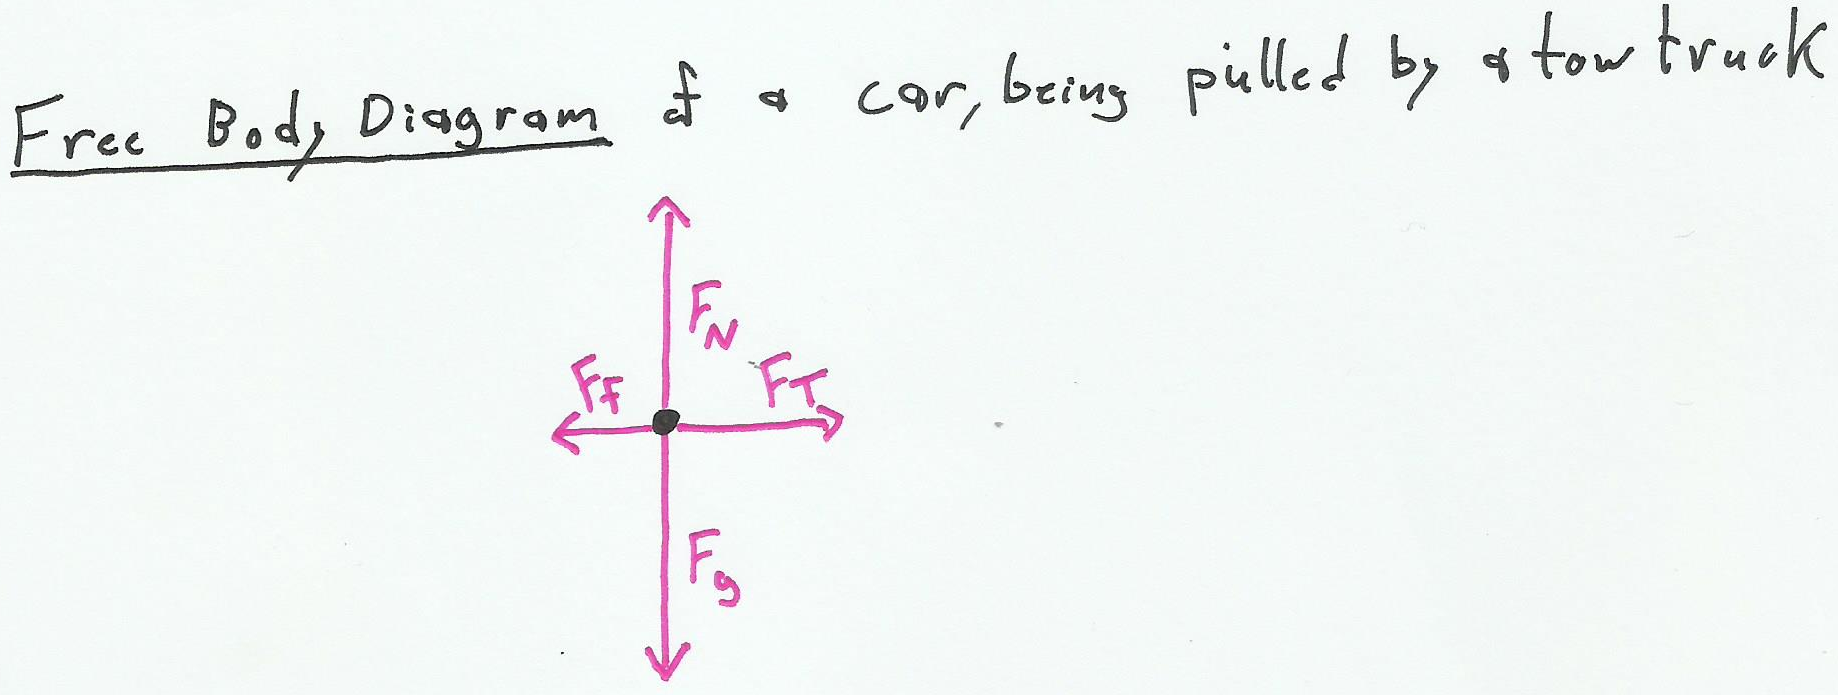
\includegraphics[width=0.7\linewidth]{CH4/CraigFBD.png}
\end{figure}
\end{frame}


\begin{frame}
\begin{figure}
    \centering
    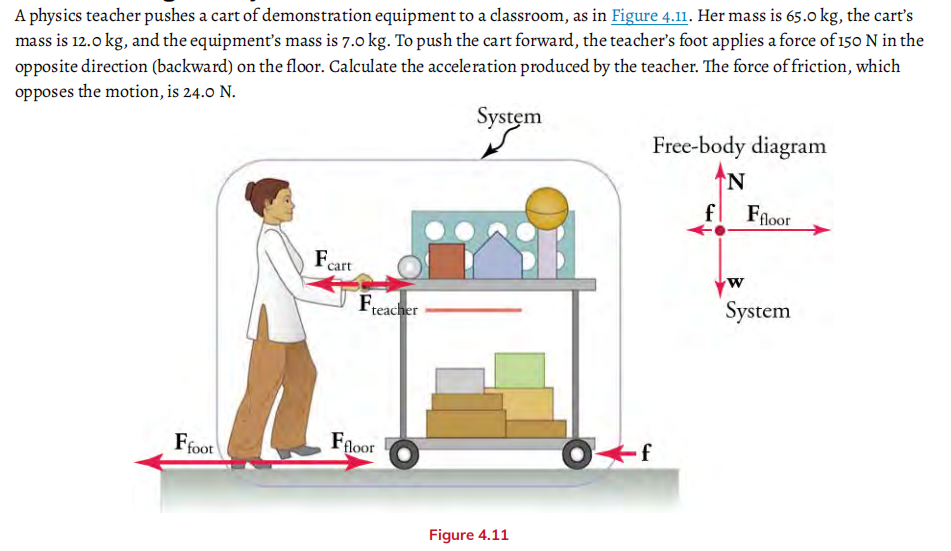
\includegraphics[width=1\linewidth]{Screenshot 2024-11-11 130750.png}
\end{figure}
\end{frame}


\begin{frame}
\frametitle{Newton's Third Law - Statement}
\begin{itemize}
    \item \textbf{Key Principle:} For every action force, there is an equal and opposite reaction force
    \item When a first body exerts a force on a second body:
    \begin{itemize}
        \item The second body exerts an equal force back
        \item The forces are equal in magnitude
        \item The forces act in opposite directions
    \end{itemize}
\end{itemize}
\end{frame}

\begin{frame}
\frametitle{Example: Physics Teacher with Cart}
\begin{block}{Problem Setup}
\begin{itemize}
    \item Teacher mass: 65.0 kg
    \item Cart mass: 12.0 kg
    \item Equipment mass: 7.0 kg
    \item Applied force: 150 N backward
    \item Friction force: 24.0 N
\end{itemize}
\end{block}
\begin{figure}[H]
    \centering
    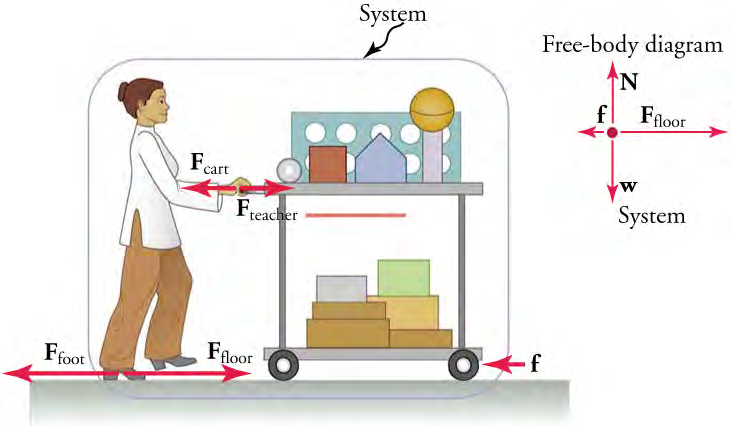
\includegraphics[width=0.5\linewidth]{CH4/Picture.png}
\end{figure}

\end{frame}

\begin{frame}
\frametitle{Solution Strategy}
\begin{itemize}
    \item Define the system:
    \begin{itemize}
        \item Teacher + Cart + Equipment
    \end{itemize}
    \item External forces:
    \begin{itemize}
        \item Floor's forward force: 150 N
        \item Friction force: -24.0 N
    \end{itemize}
    \item Net force calculation:
    \[\mathbf{F}_{\text{net}} = \mathbf{F}_{\text{floor}} - f = 150\text{ N} - 24.0\text{ N} = 126\text{ N}\]
\end{itemize}
\begin{figure}
    \centering
    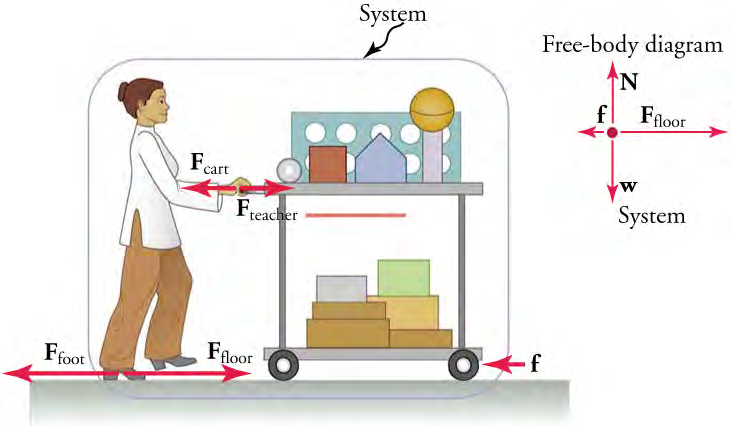
\includegraphics[width=0.5\linewidth]{CH4/Picture.png}
\end{figure}
\end{frame}

\begin{frame}
\frametitle{Common Mistakes to Avoid}
\begin{alertblock}{Important Notes}
\begin{itemize}
    \item Don't include internal forces in net force calculations
    \item Internal forces cancel out within the system
    \item Examples of internal forces:
    \begin{itemize}
        \item Force between teacher's hands and cart
        \item Force between cart and equipment
    \end{itemize}
    \item System definition is crucial for problem-solving
\end{itemize}
\end{alertblock}
\end{frame}

\begin{frame}
\frametitle{Tips for Success}
\begin{block}{Key Points}
\begin{itemize}
    \item Always identify the system clearly
    \item Draw a free-body diagram
    \item Label all external forces
    \item Remember:
    \begin{itemize}
        \item Action and reaction forces act on different objects
        \item Forces between system components cancel out
        \item Net force considers only external forces
    \end{itemize}
\end{itemize}
\end{block}
\end{frame}

\begin{frame}
\frametitle{Practice Problem}
An astronaut in space wants to move upward. Which direction should they throw an object?
\end{frame}

\begin{frame}
\begin{itemize}
    \item \textbf{Correct Answer:} Downward
    \item \textbf{Explanation:}
    \begin{itemize}
        \item Action: Astronaut throws object downward
        \item Reaction: Object pushes astronaut upward
        \item Forces are equal in magnitude, opposite in direction
    \end{itemize}
\end{itemize}
\end{frame}



\begin{frame}
\frametitle{Acknowledgments}
\begin{itemize}
    \item Original article published in Ontario Association of Physics Teachers newsletter
    \item Author: Eric Haller, Physics Teacher at Bond Schools International
    \item Reference: Knight, R.D., "FIVE EASY LESSONS: Strategies for Successful Physics Teaching"
\end{itemize}
\end{frame}

\end{document}